\chapter{Campaigns C23 and C24}\label{apx:campaigns}

This section provides an overview with representative plots of discharges over time. This section focuses on the signals used by \ac{APODIS} algorithm.

\section{Campaign C23 Overview}

\subsection{Non-disruptive Discharges}

As \autoref{fig:c23-nondisruptive-1} and \autoref{fig:c23-nondisruptive-2} show, the non-disruptive C23 campaign's discharges are characterized by a stable and predictable pattern. There are some minor differences, for example, total input power (signal 7) on discharge 74469 is degraded near second 60, or, on discharges 74473 and 74474, plasma density (signal 4) is slightly different.

\begin{figure}[H]
    \centering
    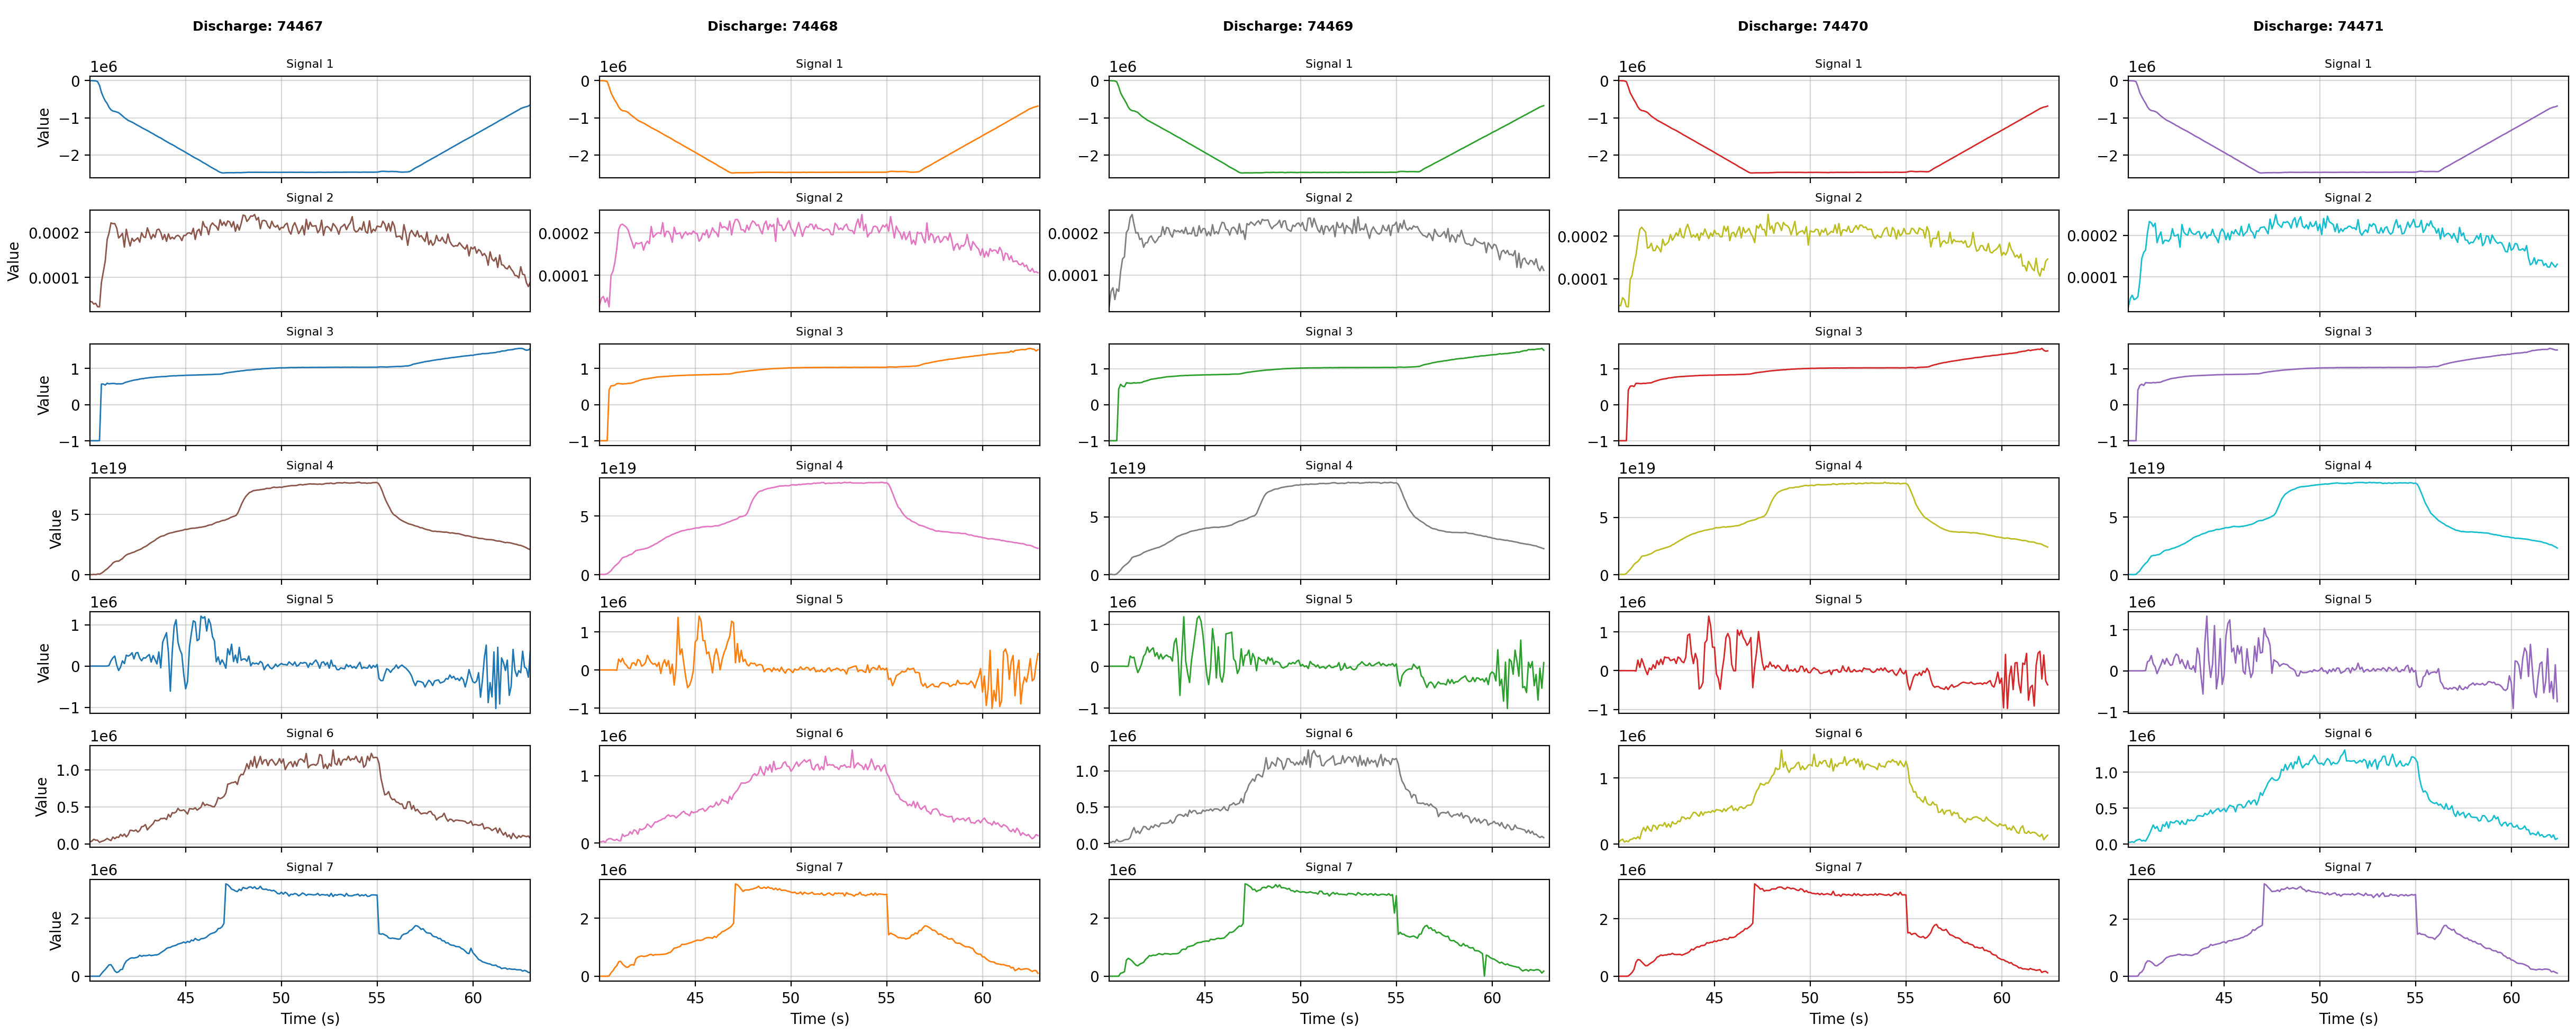
\includegraphics[width=\textwidth]{C23/C23-non-disruptive-1.png}
    \caption{Non-disruptive discharges from the C23 campaign (1)}
    \label{fig:c23-nondisruptive-1}    
\end{figure}

\begin{figure}[H]
    \centering
    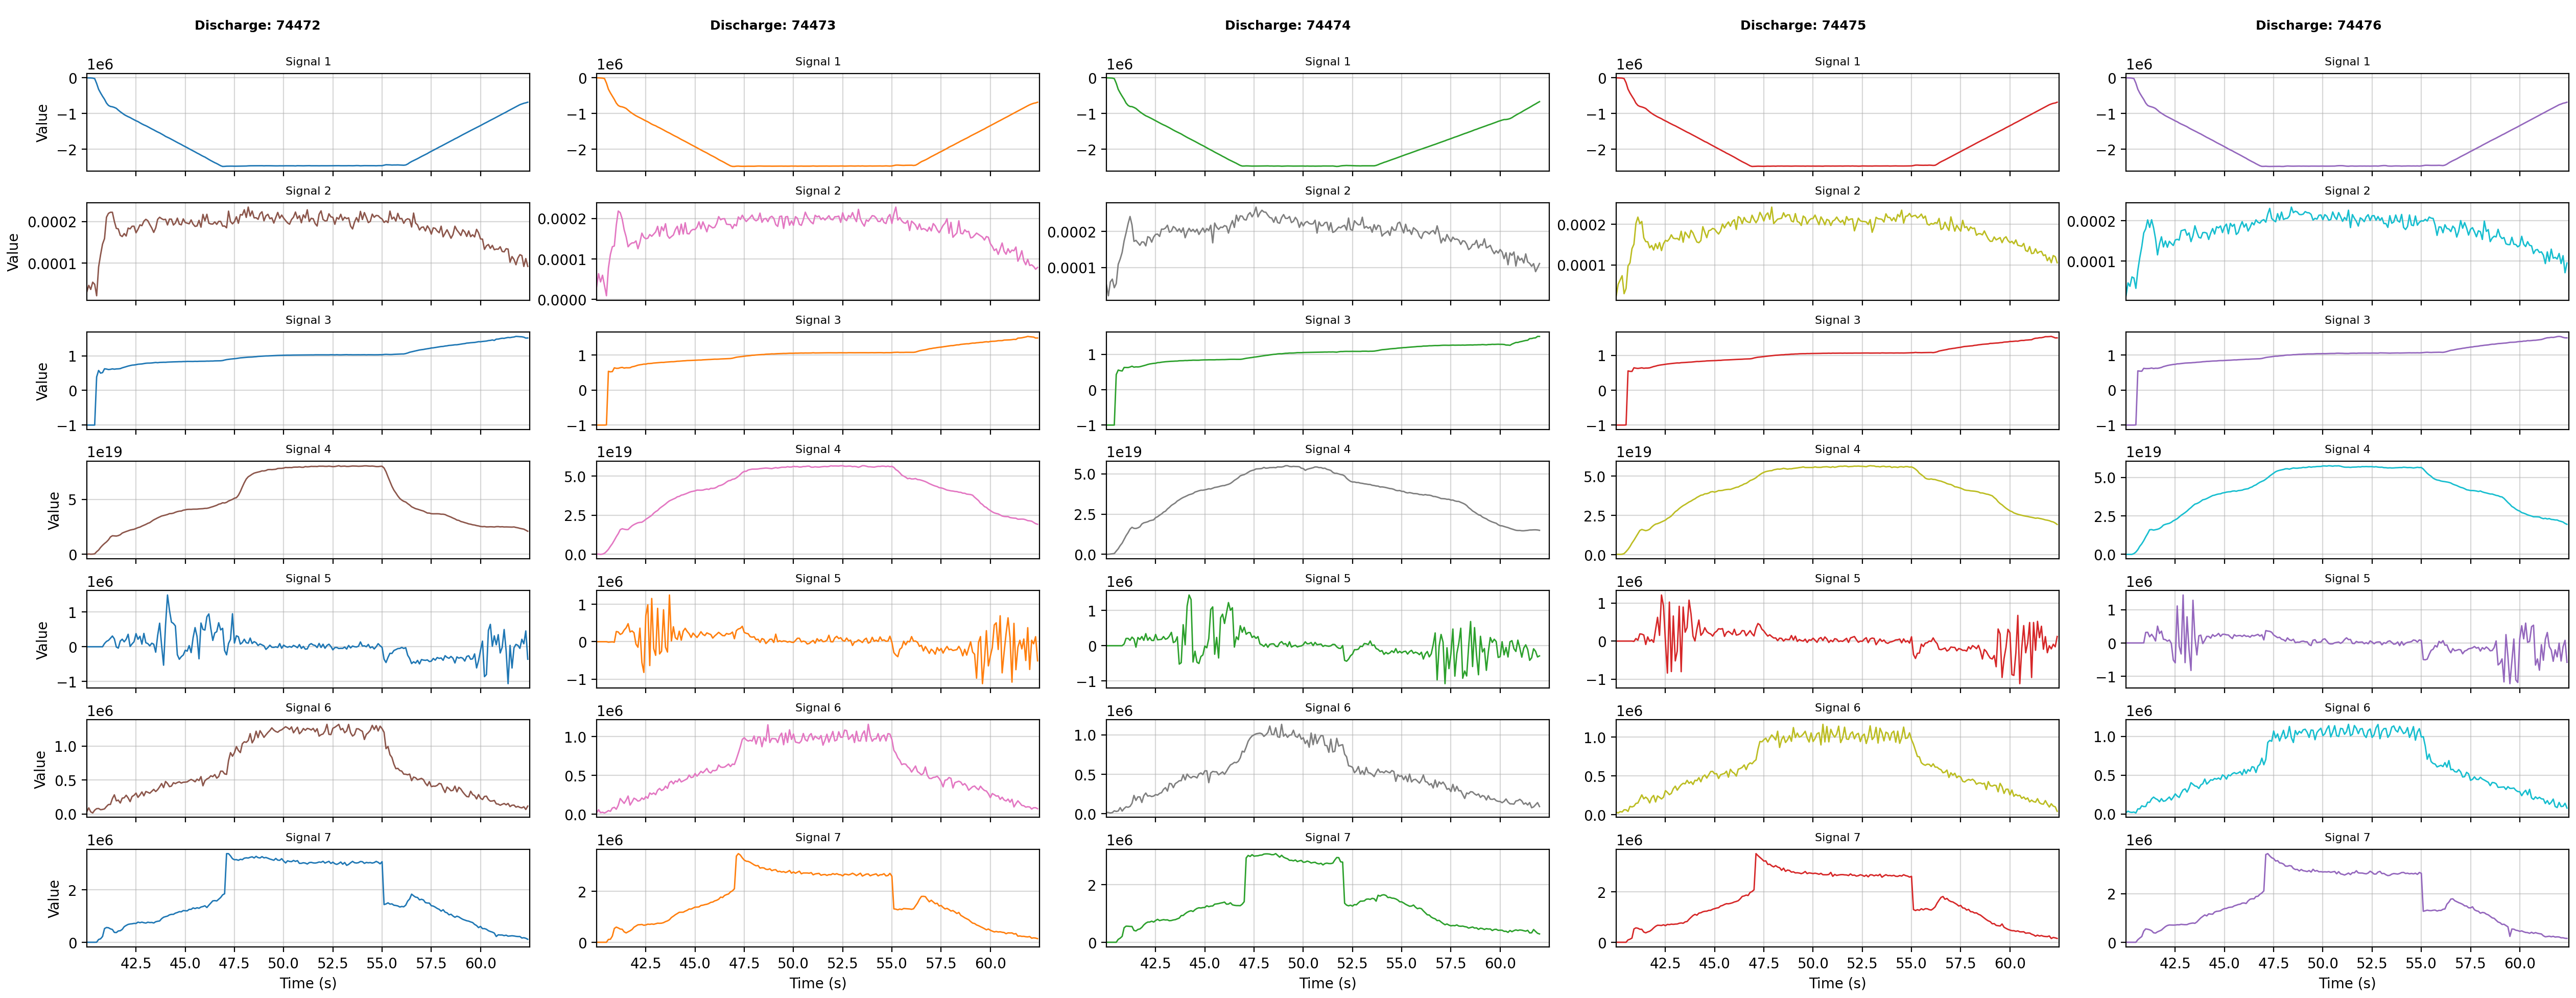
\includegraphics[width=\textwidth]{C23/C23-non-disruptive-2.png}
    \caption{Non-disruptive discharges from the C23 campaign (2)}
    \label{fig:c23-nondisruptive-2}    
\end{figure}

\subsection{Disruptive Discharges}

Disruptive discharges, as shown in \autoref{fig:c23-disruptive}, exhibit significant deviations from the expected patterns. These anomalies can be identified by abrupt changes in the signals. For comparison, the first discharge (74477) is a non-disruptive discharge, while the others are disruptive. Disruptive discharges are usually shorter than non-disruptive ones, as they are stopped to avoid damage to the machine. 

\begin{figure}[H]
    \centering
    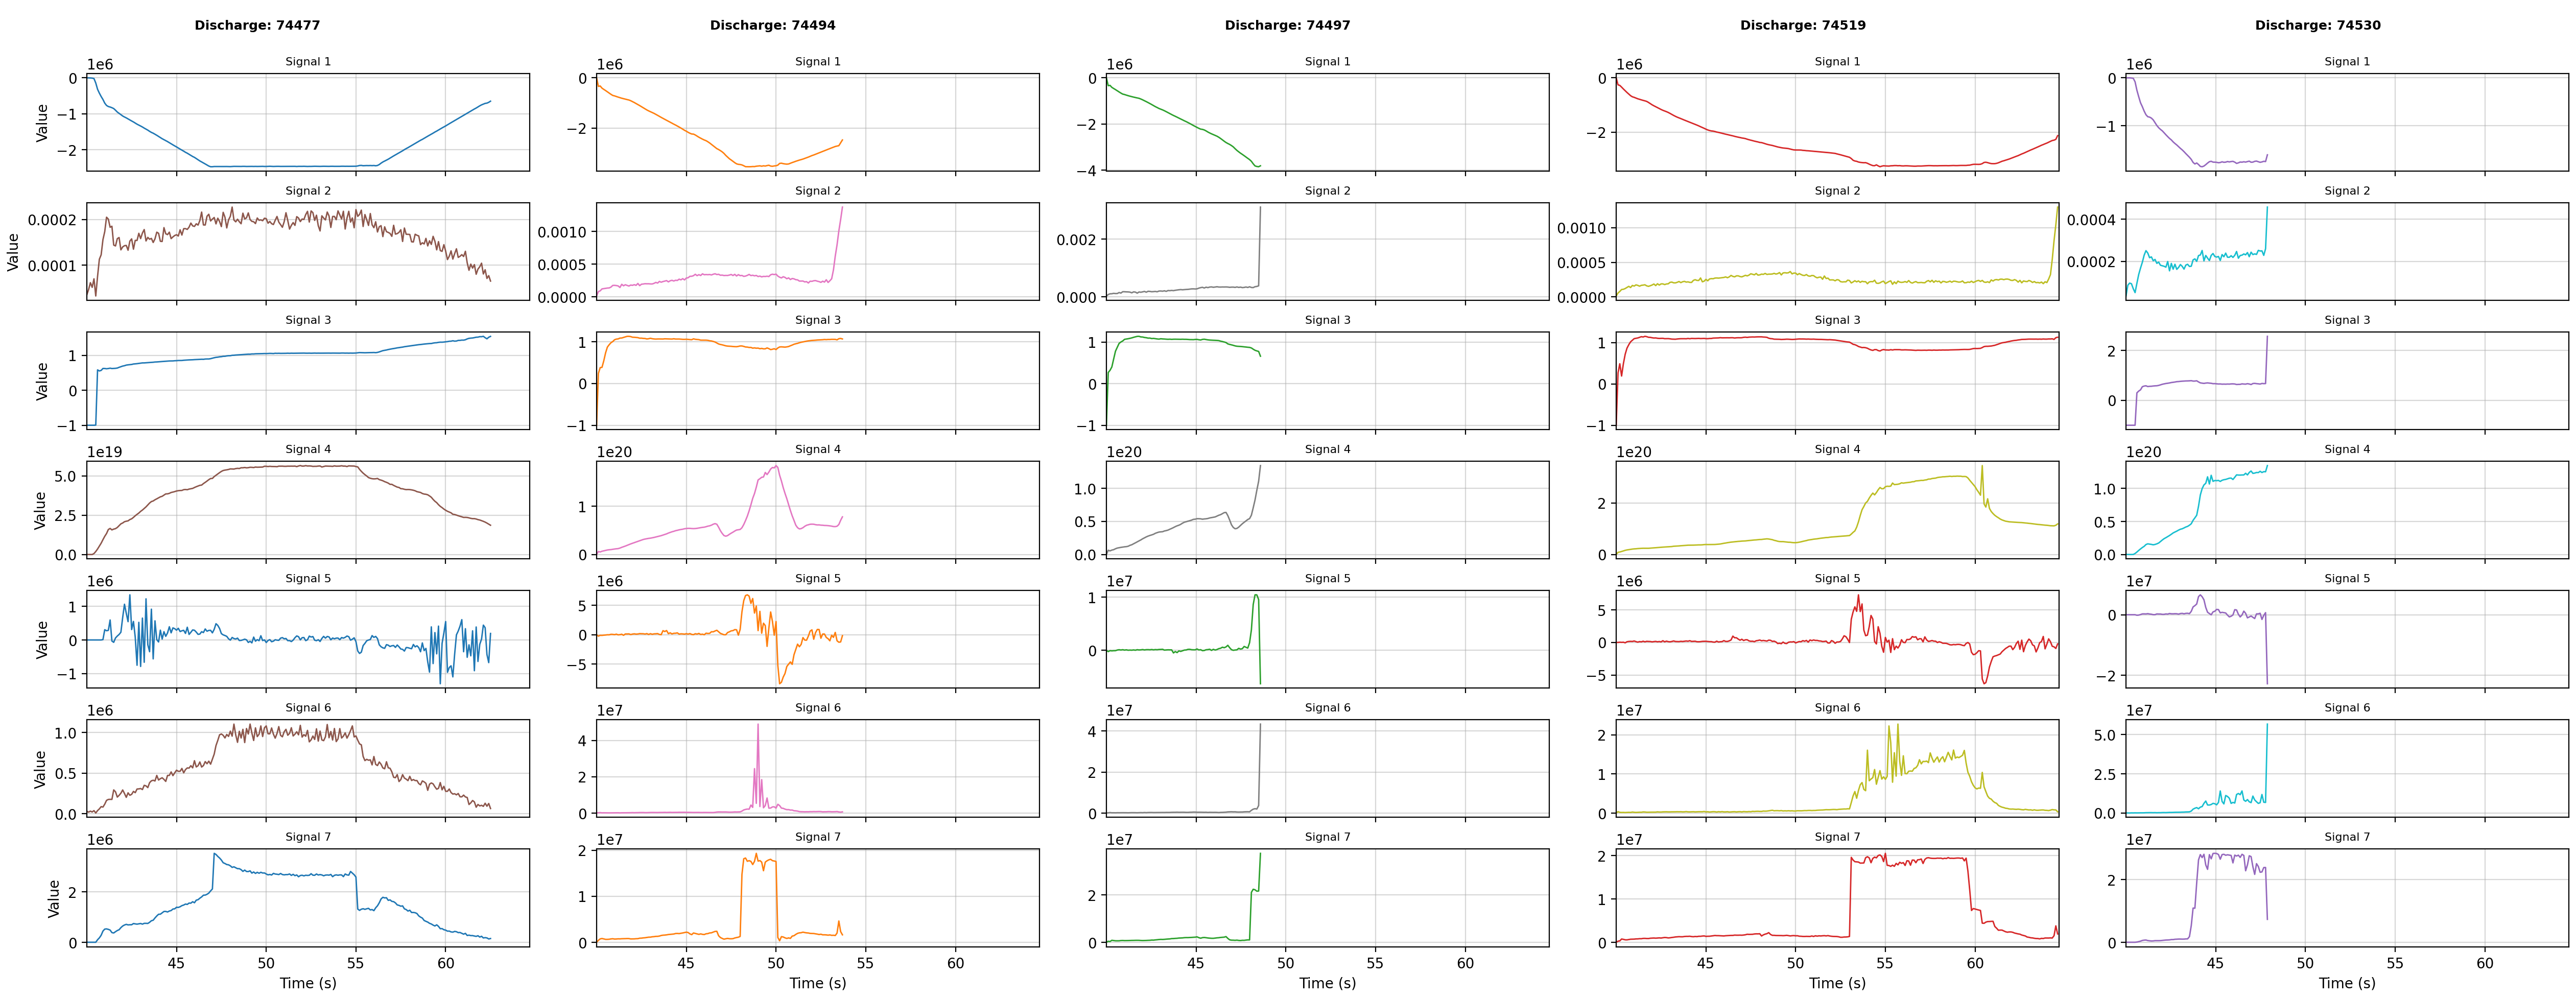
\includegraphics[width=\textwidth]{C23/C23-disruptive.png}
    \caption{Disruptive discharges from the C23 campaign}
    \label{fig:c23-disruptive}    
\end{figure}

\section{Comparison with Campaign C24}

Discharges from the C24 campaign have a slight different pattern than the C23 campaign.\ \autoref{fig:c23-vs-c24-nondisruptive} shows a comparison of plasma current (signal 1) between the two campaigns. The C23 discharge is represented on blue color, while the other signals belong to the C24 campaign. This differences on the plasma current affect to models trained on C23 campaign, and can lead to false positives when detecting anomalies.

\begin{figure}[H]
    \centering
    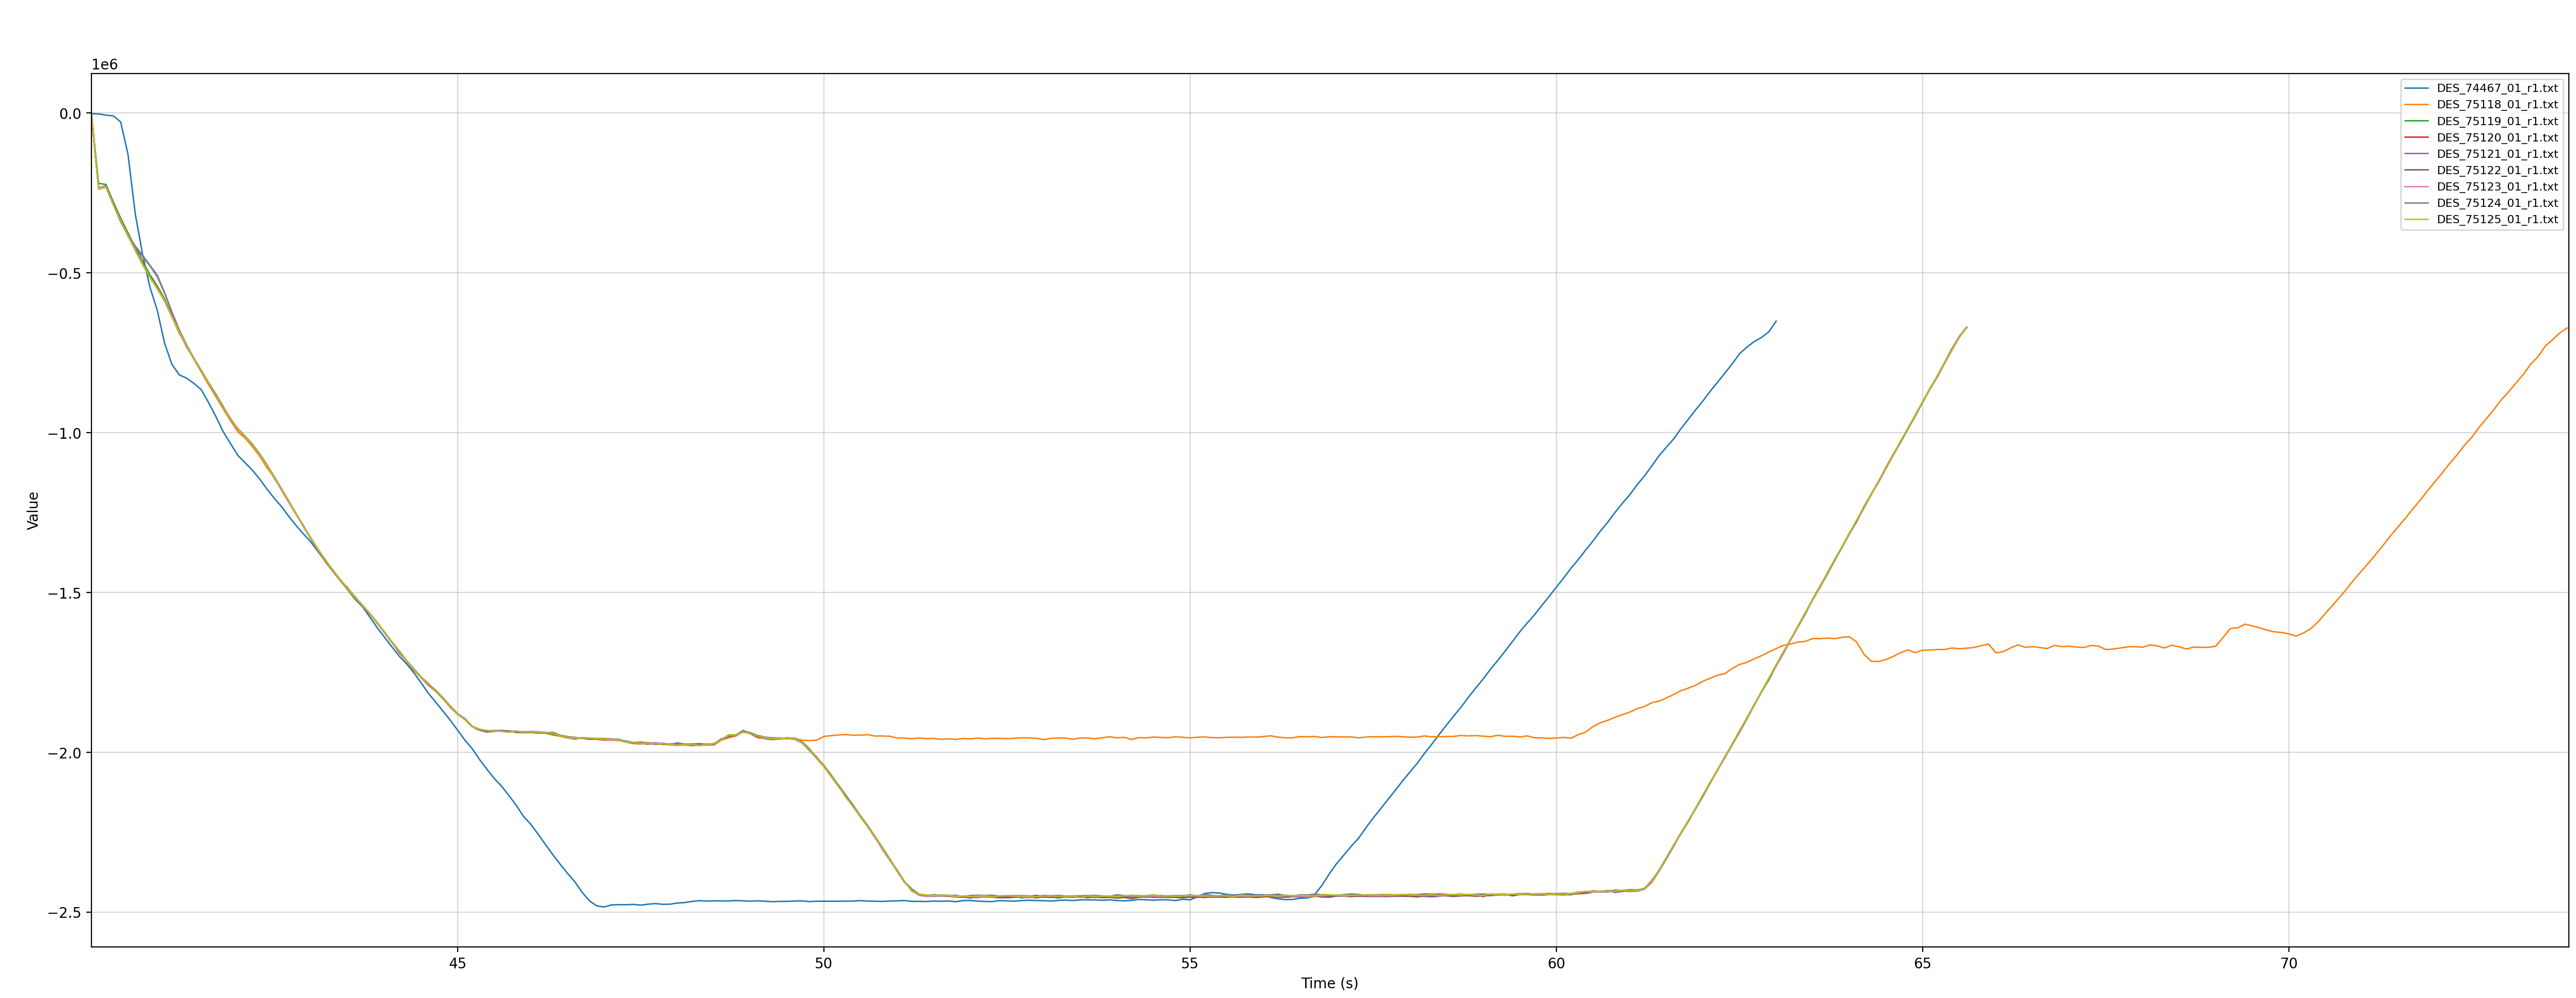
\includegraphics[width=\textwidth]{C23-vs-C24-non-disruptive.png}
    \caption{Comparison of plasma current between C23 and C24 campaigns}
    \label{fig:c23-vs-c24-nondisruptive}
\end{figure}
